\documentclass[11pt,a4paper]{article}

% ---------- Encodage & langue ----------
\usepackage[T1]{fontenc}
\usepackage[utf8]{inputenc}
\usepackage[french]{babel}
\usepackage{lmodern}

% ---------- Mise en page ----------
\usepackage[a4paper,margin=2.3cm]{geometry}
\usepackage{setspace}
\onehalfspacing

% ---------- Maths & sciences ----------
\usepackage{amsmath,amssymb}

% ---------- Tableaux, figures, code ----------
\usepackage{booktabs}
\usepackage{array}
\usepackage{graphicx}
\usepackage{float}
\usepackage{caption}
\usepackage{xcolor}
\usepackage{enumitem}
\usepackage{fancyvrb}

% ---------- Liens ----------
\usepackage[colorlinks=true,linkcolor=blue!55!black,urlcolor=blue!55!black,
            citecolor=blue!55!black]{hyperref}

% ---------- Boites d'interpretation (sans dependance lourde) ----------
\definecolor{boxgray}{RGB}{244,246,248}
\definecolor{boxline}{RGB}{90,120,150}
% Encadre gris clair avec barre laterale coloree et titre "Interprétation".
\newenvironment{interpret}{%
  \par\medskip\noindent
  \setlength{\fboxsep}{8pt}%
  \begin{lrbox}{\interpretbox}%
  \begin{minipage}{\dimexpr\linewidth-2\fboxsep-4pt\relax}%
  \textbf{\textcolor{boxline}{Interprétation.}}\;\ignorespaces
}{%
  \end{minipage}%
  \end{lrbox}%
  \noindent\textcolor{boxline}{\rule{3pt}{\dimexpr\ht\interpretbox+\dp\interpretbox\relax}}%
  \colorbox{boxgray}{\usebox{\interpretbox}}%
  \par\medskip
}
\newsavebox{\interpretbox}

\captionsetup{font=small,labelfont=bf}

\title{\textbf{Projet individuel --- Algèbre Linéaire Numérique\\
Appliquée à l'Analyse de Données}\\[4pt]
\large Compte rendu}
\author{Hazem Douzi}
\date{\today}

\begin{document}
\maketitle

\begin{abstract}
\noindent Ce rapport présente la résolution des trois exercices du projet, accompagnés des
résultats numériques obtenus dans le notebook \texttt{hazem\_douzi.ipynb}, des visualisations
produites, de leur interprétation et d'une conclusion. On y traite : (1)~la résolution de
systèmes linéaires $Ax=b$ par méthodes directes (LU, Cholesky) et itératives (Jacobi,
Gauss--Seidel) ; (2)~les décompositions SVD et QR ; (3)~les applications à l'analyse de
données (ACP et compression d'image). L'exercice~4 rassemble les questions de synthèse.
Tous les calculs utilisent une graine aléatoire fixe (\verb|np.random.seed|), les résultats
sont donc \textbf{reproductibles}.
\end{abstract}

{\small\tableofcontents}
\bigskip

% =====================================================================
\section{Introduction}
L'objectif du projet est de mettre en pratique les outils d'algèbre linéaire numérique de
\texttt{numpy} et \texttt{scipy} et de les appliquer à l'analyse de données. Pour chaque
question, on rappelle l'objectif, on présente les résultats du notebook, puis on les
\emph{interprète}. Les bibliothèques utilisées sont \texttt{numpy}, \texttt{scipy} et
\texttt{matplotlib}.

% =====================================================================
\section{Exercice 1 --- Résolution de systèmes linéaires}

On résout $Ax=b$ avec $A$ une matrice $4\times4$ \textbf{symétrique définie positive (SDP)}.
On compare des méthodes \emph{directes} (LU, Cholesky), exactes à l'arrondi près, et des
méthodes \emph{itératives} (Jacobi, Gauss--Seidel), qui approchent la solution.

\subsection{Méthode directe : décomposition LU}

\subsubsection{Construction d'une matrice SDP}
Une matrice est SDP si $A=A^{\top}$ et $x^{\top}Ax>0$ pour tout $x\neq 0$, ce qui équivaut à
\textbf{toutes ses valeurs propres strictement positives}. On construit $A = B^{\top}B + 4I$
(avec $B$ aléatoire) : $B^{\top}B$ est toujours symétrique semi-définie positive, et le
terme $+4I$ rend toutes les valeurs propres strictement positives.

\[
A=\begin{bmatrix}
 4.581 & -0.731 & -0.248 & 0.659\\
-0.731 & 8.029 & 2.590 & 0.433\\
-0.248 & 2.590 & 10.104 & 3.384\\
 0.659 & 0.433 & 3.384 & 7.442
\end{bmatrix},\qquad
b=\begin{bmatrix}-1.013\\0.314\\-0.908\\-1.412\end{bmatrix}.
\]

\begin{table}[H]\centering
\caption{Valeurs propres de $A$ et test de symétrie.}
\begin{tabular}{lccccc}
\toprule
Valeurs propres & $13.484$ & $7.708$ & $4.117$ & $4.846$ & \\
\midrule
Toutes $>0$ ? & \multicolumn{4}{c}{Oui} & $A=A^{\top}$ : \textbf{Vrai}\\
\bottomrule
\end{tabular}
\end{table}

\begin{interpret}
Les quatre valeurs propres sont strictement positives et $A$ est symétrique : $A$ est bien
\textbf{SDP}. Cela légitime l'emploi de Cholesky (\S2.2) en complément de LU.
\end{interpret}

\subsubsection{Factorisation LU avec \texttt{scipy.linalg.lu}}
\verb|scipy.linalg.lu(A)| renvoie $P$ (permutation), $L$ (triangulaire inférieure à diagonale
unité) et $U$ (triangulaire supérieure), avec la convention $A=PLU$, donc $P^{\top}A = LU$.

\begin{table}[H]\centering
\caption{Matrices $L$ et $U$ obtenues ($P=I$ : aucun échange de lignes nécessaire).}
\begin{tabular}{cc}
\toprule
$L$ & $U$\\
\midrule
$\begin{bmatrix}
1 & 0 & 0 & 0\\
-0.160 & 1 & 0 & 0\\
-0.054 & 0.322 & 1 & 0\\
0.144 & 0.068 & 0.350 & 1
\end{bmatrix}$
&
$\begin{bmatrix}
4.581 & -0.731 & -0.248 & 0.659\\
0 & 7.912 & 2.550 & 0.538\\
0 & 0 & 9.268 & 3.246\\
0 & 0 & 0 & 6.173
\end{bmatrix}$\\
\bottomrule
\end{tabular}
\end{table}

\noindent Vérification : $P^{\top}A = LU \Rightarrow$ \textbf{Vrai}.

\subsubsection{Résolution par substitutions triangulaires}
Une fois $A=PLU$, résoudre $Ax=b$ revient à deux systèmes triangulaires peu coûteux :
\[
\tilde b = P^{\top}b,\qquad Ly=\tilde b\ \text{(substitution avant)},\qquad
Ux=y\ \text{(substitution arrière)}.
\]
On obtient
\[
x \approx (-0.195056,\ 0.047759,\ -0.056848,\ -0.149426).
\]

\subsubsection{Vérification avec \texttt{numpy.linalg.solve}}
La routine \verb|numpy.linalg.solve| (LAPACK) sert de référence. Le test \verb|np.allclose|
renvoie \textbf{Vrai} : notre résolution coïncide avec la référence à la précision machine.

\subsection{Méthode de Cholesky}
Comme $A$ est SDP, on peut écrire $A=LL^{\top}$. La résolution via \verb|cho_factor| /
\verb|cho_solve| donne la \textbf{même} solution que LU. On compare ensuite temps et précision
(résidu $\lVert Ax-b\rVert_2$, moyenné sur $1000$ répétitions).

\begin{table}[H]\centering
\caption{Comparaison LU vs Cholesky (temps indicatif, dépend de la machine).}
\begin{tabular}{lcc}
\toprule
 & \textbf{LU} & \textbf{Cholesky}\\
\midrule
Temps moyen ($\mu s$) & $\approx 35$ & $\approx 10$\\
Résidu $\lVert Ax-b\rVert_2$ & $2.29\times10^{-16}$ & $4.00\times10^{-16}$\\
\bottomrule
\end{tabular}
\end{table}

\begin{interpret}
\textbf{Précision} : les deux résidus sont de l'ordre de $10^{-16}$, soit la précision machine
($\varepsilon_{\text{mach}}\approx2.2\times10^{-16}$) ; l'écart est négligeable.
\textbf{Temps} : Cholesky est ici $\sim$2--3 fois plus rapide que LU car il exploite la symétrie
et évite le pivotage. \textbf{Règle pratique} : dès que $A$ est SDP, on préfère Cholesky.
\end{interpret}

\subsection{Méthodes itératives : Jacobi et Gauss--Seidel}
On décompose $A=D+(L+U)$ ($D$ diagonale, $L$/$U$ parties triangulaires strictes).
\begin{itemize}[nosep]
\item \textbf{Jacobi} (mise à jour \emph{simultanée}) : $x^{(k+1)} = D^{-1}\big(b-(L+U)\,x^{(k)}\big)$.
\item \textbf{Gauss--Seidel} (mise à jour \emph{séquentielle}) : pour calculer $x_i^{(k+1)}$, on
réutilise immédiatement les composantes déjà recalculées $x_1^{(k+1)},\dots,x_{i-1}^{(k+1)}$.
\end{itemize}
Critère d'arrêt : $\lVert x^{(k+1)}-x^{(k)}\rVert_2 < \text{tol}=10^{-6}$ (au plus $100$ itérations).

\begin{table}[H]\centering
\caption{Résultats des méthodes itératives (convergence vers la solution de LU).}
\begin{tabular}{lcc}
\toprule
 & \textbf{Jacobi} & \textbf{Gauss--Seidel}\\
\midrule
Nombre d'itérations & $19$ & $\mathbf{10}$\\
Résidu final $\lVert Ax-b\rVert_2$ & $3.90\times10^{-6}$ & $1.56\times10^{-7}$\\
Solution & \multicolumn{2}{c}{identique à LU}\\
\bottomrule
\end{tabular}
\end{table}

\begin{table}[H]\centering
\caption{Norme de la correction $\lVert x^{(k+1)}-x^{(k)}\rVert_2$ à quelques itérations.}
\begin{tabular}{cccccc}
\toprule
Itération & 1 & 5 & 8 & 10 & 19\\
\midrule
Jacobi & $0.3074$ & $0.0100$ & $0.00135$ & $0.000354$ & $9\times10^{-7}$\\
Gauss--Seidel & $0.2740$ & $0.000814$ & $6\times10^{-6}$ & $\le10^{-6}$ (convergé) & ---\\
\bottomrule
\end{tabular}
\end{table}

\begin{figure}[H]\centering
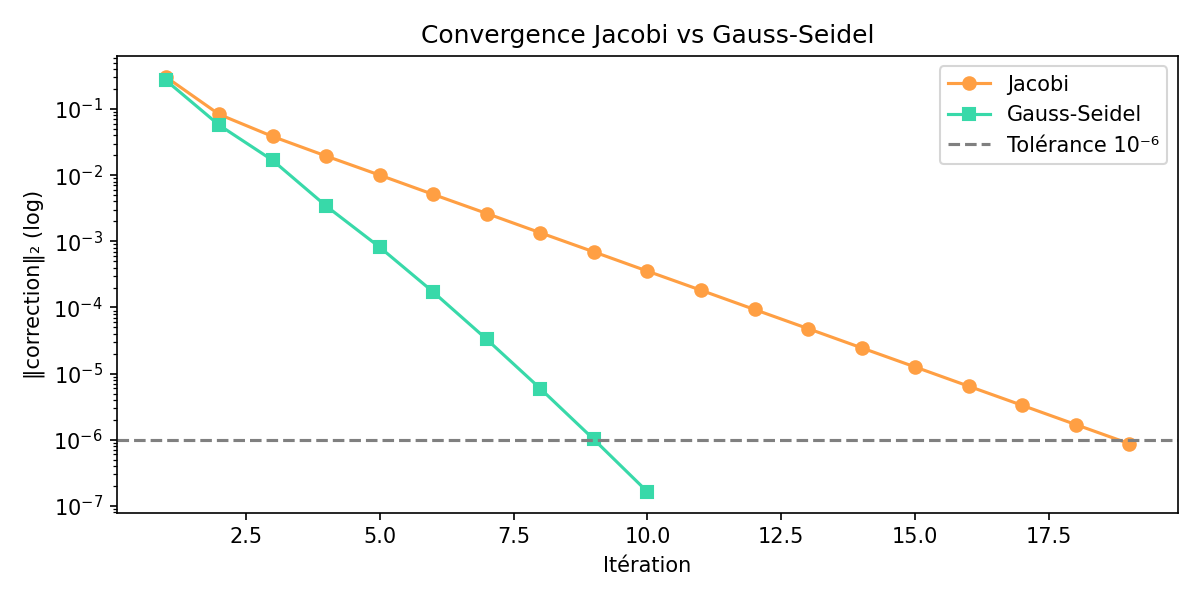
\includegraphics[width=0.8\textwidth]{convergence.png}
\caption{Convergence comparée de Jacobi et Gauss--Seidel (échelle logarithmique).
Gauss--Seidel atteint la tolérance $10^{-6}$ en deux fois moins d'itérations.}
\end{figure}

\begin{interpret}
Gauss--Seidel converge en \textbf{10} itérations contre \textbf{19} pour Jacobi ($\sim$2$\times$
moins), avec un résidu final plus faible. Sa pente de convergence est plus raide car il exploite
l'information « fraîche » à chaque pas. La convergence des deux méthodes est ici garantie : $A$
est SDP et à diagonale dominante.
\end{interpret}

% =====================================================================
\section{Exercice 2 --- Décompositions SVD et QR}

\subsection{Décomposition en valeurs singulières (SVD)}

\subsubsection{Matrice de données}
On simule les notes de $10$ étudiants sur $5$ matières (entiers de $0$ à $19$) :
\[
D=\begin{bmatrix}
12&15&0&3&3\\7&9&19&18&4\\6&12&1&6&7\\14&17&5&13&8\\9&19&16&19&5\\
15&15&0&18&3\\17&19&19&19&14\\7&0&1&9&0\\10&3&11&18&2\\0&0&4&5&6
\end{bmatrix}.
\]

\subsubsection{Calcul et reconstruction}
\verb|numpy.linalg.svd| (option \verb|full_matrices=False|) donne $D=U\Sigma V^{\top}$ avec
$U\in\mathbb{R}^{10\times5}$, $\Sigma$ de taille $5$ et $V^{\top}\in\mathbb{R}^{5\times5}$.

\begin{table}[H]\centering
\caption{Valeurs singulières de $D$ et énergie associée.}
\begin{tabular}{lccccc}
\toprule
$\sigma_i$ & $74.73$ & $22.62$ & $14.70$ & $8.72$ & $6.31$\\
\midrule
\multicolumn{6}{l}{$\sigma_1$ concentre $\dfrac{\sigma_1^2}{\sum_i\sigma_i^2}\approx \mathbf{86.9\,\%}$
de l'énergie.}\\
\bottomrule
\end{tabular}
\end{table}

\noindent Reconstruction complète : $\lVert D - D_{\text{rec}}\rVert_F \approx 5.8\times10^{-14}$
(\verb|np.allclose| $\Rightarrow$ \textbf{Vrai}) : la SVD reconstruit $D$ \textbf{exactement}.

\subsubsection{Approximation de rang 2 (Eckart--Young)}
En ne gardant que les deux plus grandes valeurs singulières
$D_2=U_{:,:2}\,\mathrm{diag}(\sigma_{1:2})\,V^{\top}_{:2,:}$, on obtient l'erreur relative de
Frobenius :
\[
\frac{\lVert D - D_2\rVert_F}{\lVert D\rVert_F}\approx \mathbf{22.7\,\%}.
\]
\begin{interpret}
D'après le théorème d'\textbf{Eckart--Young}, $D_2$ est la meilleure approximation de rang~2.
Avec seulement \textbf{2 composantes sur 5}, on conserve $\approx 95\,\%$ de l'énergie
($1-0.227^2\approx 0.95$) : excellent compromis taille/fidélité, qui motive la réduction de
dimension de l'ACP.
\end{interpret}

\subsection{Décomposition QR}
\verb|scipy.linalg.qr(D)| factorise $D=QR$ avec $Q$ orthogonale ($10\times10$) et $R$
triangulaire supérieure ($10\times5$). Pivots (diagonale de $R$) :
$(-34.19,\,-15.65,\,24.00,\,-11.78,\,9.03)$.

\begin{table}[H]\centering
\caption{Vérifications de la décomposition QR.}
\begin{tabular}{lc}
\toprule
Propriété & Résultat\\
\midrule
$Q^{\top}Q = I$ (colonnes orthonormées) & \textbf{Vrai}\\
$QR = D$ & \textbf{Vrai}\\
\bottomrule
\end{tabular}
\end{table}

\begin{interpret}
$Q$ est bien orthogonale et $QR$ restitue exactement $D$. La QR est l'outil de référence pour les
\textbf{moindres carrés} et la \textbf{stabilité numérique} (orthogonalisation des colonnes).
\end{interpret}

% =====================================================================
\section{Exercice 3 --- Application à l'analyse de données}

\subsection{Analyse en Composantes Principales (ACP)}
On applique l'ACP à $D$ : (1) centrage, (2) SVD de la matrice centrée, (3) projection sur les
premières composantes principales.

\subsubsection{Centrage}
On soustrait la moyenne de chaque colonne. Moyennes par matière :
$(9.7,\,10.9,\,7.6,\,12.8,\,5.2)$ ; après centrage, chaque colonne est de moyenne nulle
(à l'arrondi près). Le centrage est indispensable car l'ACP analyse la variance \emph{autour de
la moyenne}.

\subsubsection{SVD des données centrées et variance expliquée}
Les lignes de $V^{\top}$ sont les composantes principales (CP) ; $\sigma_i^2$ est proportionnel
à la variance portée par la CP$_i$.

\begin{table}[H]\centering
\caption{Variance expliquée par chaque composante principale.}
\begin{tabular}{lccccc}
\toprule
Composante & CP1 & CP2 & CP3 & CP4 & CP5\\
\midrule
$\sigma_i$ (centré) & $32.07$ & $22.22$ & $13.71$ & $8.15$ & $6.01$\\
Variance (\%) & $56.7$ & $27.2$ & $10.4$ & $3.7$ & $2.0$\\
Cumulée (\%) & $56.7$ & $\mathbf{84.0}$ & $94.3$ & $98.0$ & $100$\\
\bottomrule
\end{tabular}
\end{table}

\subsubsection{Projection sur le plan (CP1, CP2)}
$Z = D_{\text{centré}}\,V_{:,:2}$ donne les coordonnées des étudiants :

\begin{table}[H]\centering
\caption{Coordonnées des $10$ étudiants dans le plan CP1/CP2.}
\begin{tabular}{lrr@{\qquad}lrr}
\toprule
Étudiant & CP1 & CP2 & Étudiant & CP1 & CP2\\
\midrule
Ét.1 & $7.17$ & $-10.27$ & Ét.6 & $-1.27$ & $-7.52$\\
Ét.2 & $-7.42$ & $10.34$ & Ét.7 & $-18.07$ & $-1.02$\\
Ét.3 & $7.56$ & $-5.10$ & Ét.8 & $13.25$ & $4.11$\\
Ét.4 & $-3.50$ & $-7.47$ & Ét.9 & $-0.09$ & $8.83$\\
Ét.5 & $-11.97$ & $1.32$ & Ét.10 & $14.34$ & $6.76$\\
\bottomrule
\end{tabular}
\end{table}

\begin{figure}[H]\centering
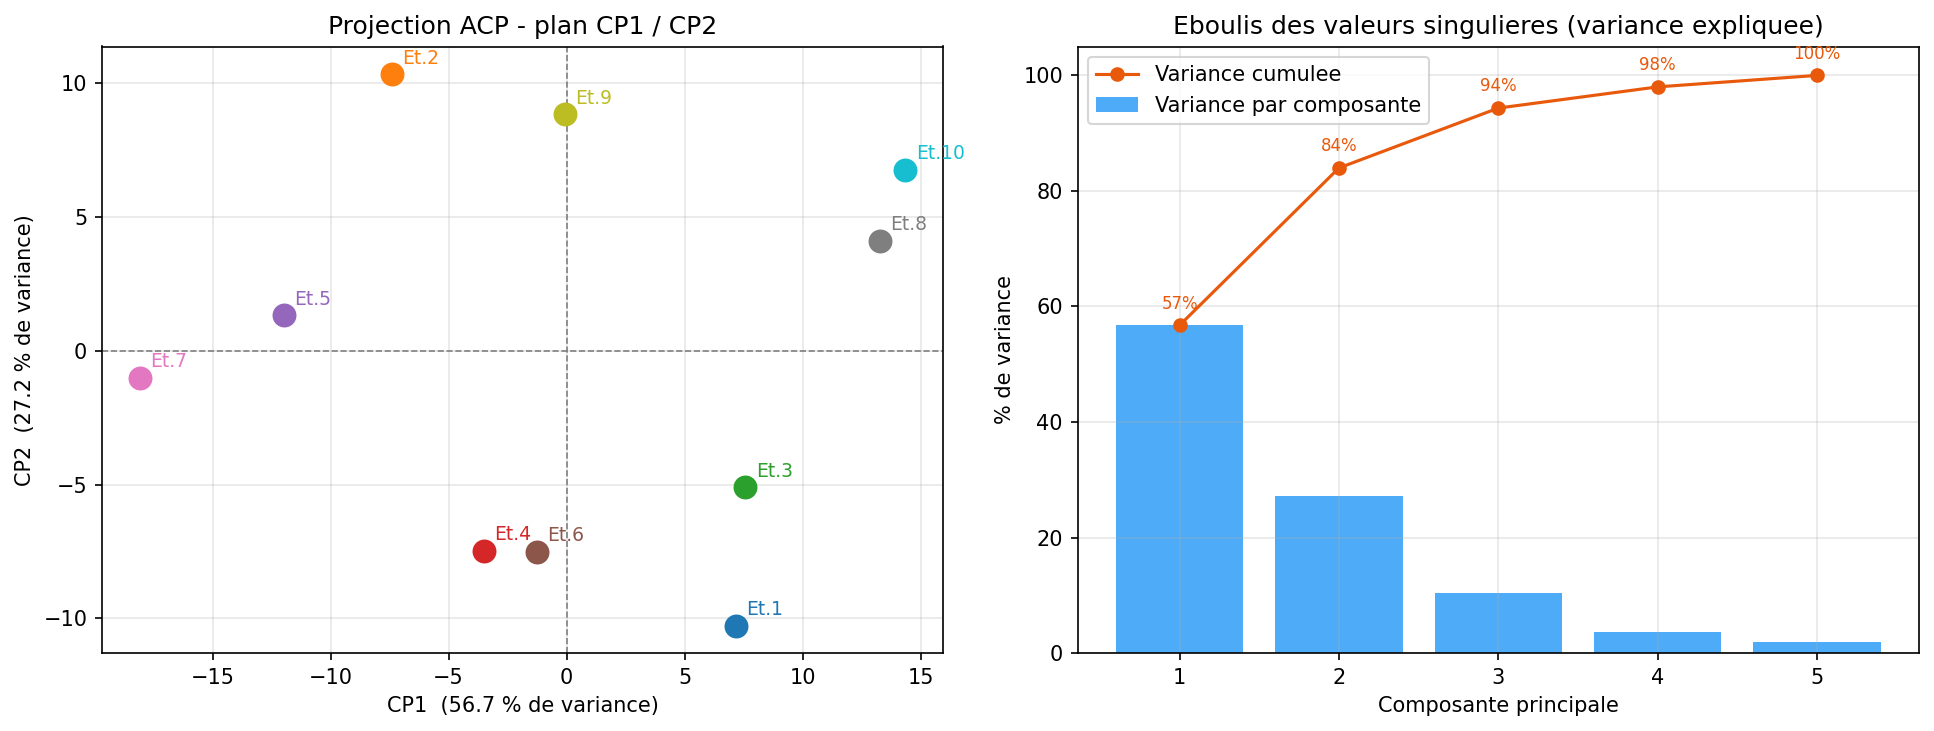
\includegraphics[width=\textwidth]{acp_visualisation.png}
\caption{À gauche : projection des étudiants dans le plan CP1/CP2. À droite : éboulis des valeurs
singulières (variance expliquée par composante et cumulée).}
\end{figure}

\begin{interpret}
\textbf{CP1 ($\approx$56.7\,\%) = niveau général.} Tous les coefficients de l'axe sont de même
signe : l'axe oppose les étudiants forts aux faibles. L'étudiant~7 (notes $[17,19,19,19,14]$, le
meilleur) se trouve à l'extrême gauche, l'étudiant~10 ($[0,0,4,5,6]$, le plus faible) à l'extrême
droite.\\[2pt]
\textbf{CP2 ($\approx$27.2\,\%) = contraste entre matières} (matières~1--2 contre matières~3--4) :
à niveau global comparable, il sépare les profils « forts dans certaines matières / faibles dans
d'autres » (ex.\ l'étudiant~2 $[7,9,19,18,4]$ s'oppose à l'étudiant~1 $[12,15,0,3,3]$).\\[2pt]
L'éboulis confirme que \textbf{2 composantes} suffisent (84\,\% de variance cumulée) : la
projection 2D est fidèle.
\end{interpret}

\subsection{Compression d'image par SVD}
Une image en niveaux de gris est une matrice de pixels. En gardant les $k$ premières valeurs
singulières, on ne stocke que $k\,(m+n+1)$ nombres au lieu de $m\times n$. On charge l'image
(fichier local \verb|image.png| sinon photo d'exemple de matplotlib, $600\times512$), on la
convertit en niveaux de gris (pondération ITU-R BT.601), puis on applique la SVD.

\begin{table}[H]\centering
\caption{Qualité vs taux de stockage selon le rang $k$ (PSNR : plus élevé = meilleur).
$\sigma_1$ capte déjà $\approx$73\,\% de l'énergie de l'image.}
\begin{tabular}{rccc}
\toprule
Rang $k$ & Stockage (\%) & $\lVert\text{erreur}\rVert_F$ & PSNR (dB)\\
\midrule
$10$ & $3.6$ & $58.85$ & $19.48$\\
$50$ & $18.1$ & $24.29$ & $27.17$\\
$100$ & $36.2$ & $13.95$ & $31.98$\\
$512$ (complet) & $185.5$ & $\approx 0$ & $\infty$\\
\bottomrule
\end{tabular}
\end{table}

\begin{figure}[H]\centering
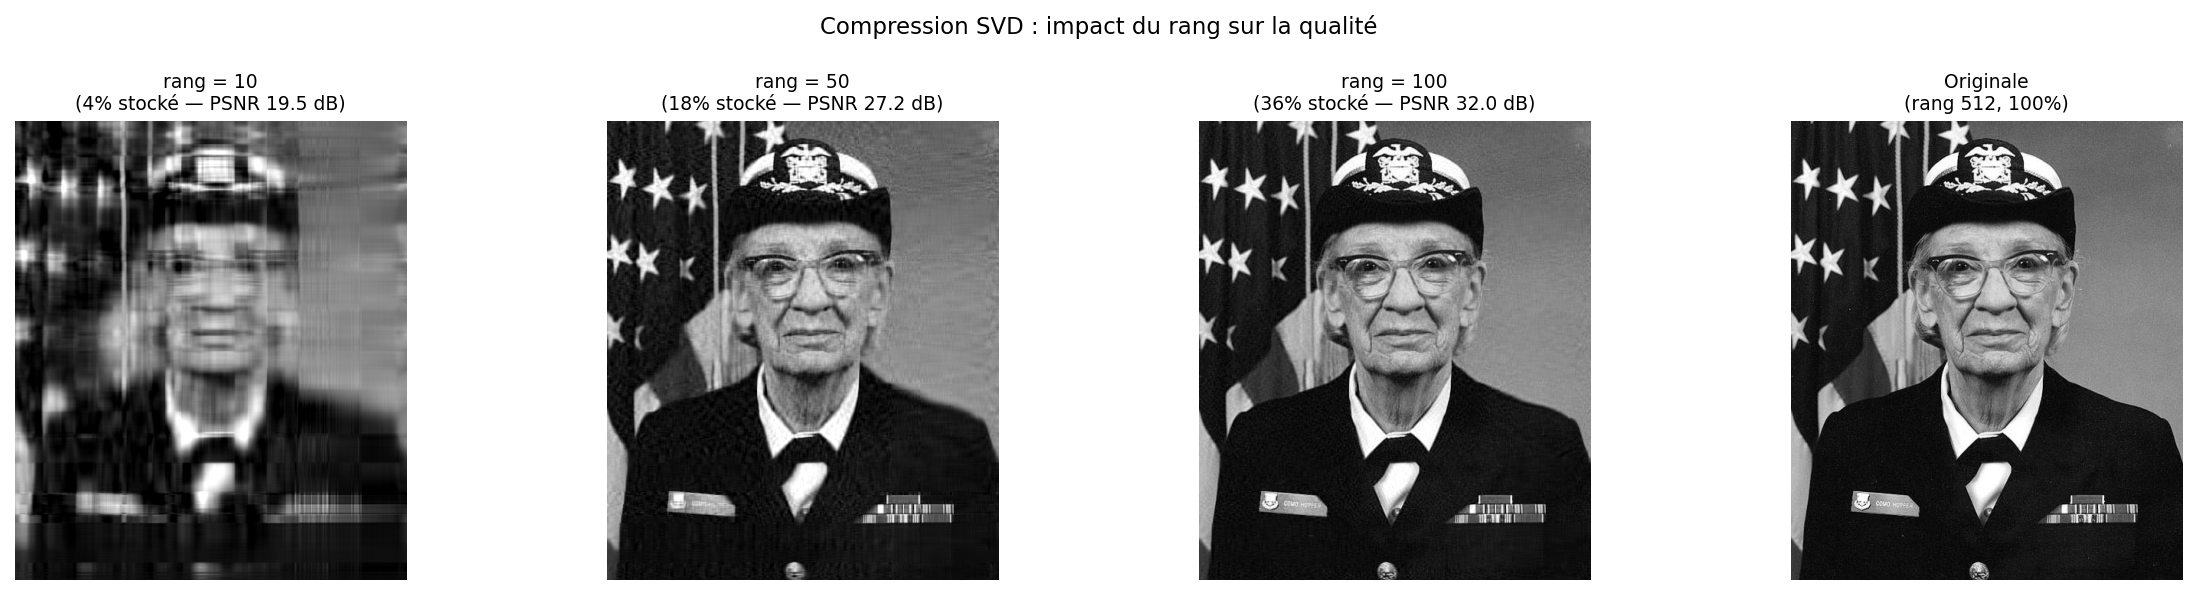
\includegraphics[width=\textwidth]{compression_svd.png}
\caption{Compression SVD : impact du rang sur la qualité visuelle (rangs 10, 50, 100 et image
originale).}
\end{figure}

\begin{interpret}
\textbf{rang 10} ($\sim$3.6\,\% de stockage) : seules les grandes structures subsistent, image
floue (PSNR $\sim$19.5\,dB), bonne uniquement pour une vignette. \textbf{rang 50} ($\sim$18\,\%) :
image reconnaissable, PSNR $\sim$27\,dB. \textbf{rang 100} ($\sim$36\,\%) : bonne qualité visuelle,
PSNR $\sim$32\,dB, compression $\sim$3$\times$. Un PSNR $>30$\,dB est généralement jugé « bonne
qualité ». À noter : stocker la SVD \emph{complète} (rang 512) coûte \emph{plus} que l'image
d'origine ($\sim$185\,\%) ; tout l'intérêt est donc de \textbf{tronquer}.
\end{interpret}

% =====================================================================
\section{Exercice 4 --- Questions de synthèse}

\subsection*{1. Performances (temps, précision) : méthodes directes vs itératives}
\textbf{Précision.} Les méthodes directes (LU, Cholesky) atteignent la \textbf{précision machine}
(résidu $\approx 2$--$4\times10^{-16}\approx\varepsilon_{\text{mach}}$) : elles résolvent le
système exactement à l'arrondi flottant près. Les méthodes itératives s'arrêtent dès que la
correction passe sous $\varepsilon=10^{-6}$, d'où un résidu plus élevé ($3.9\times10^{-6}$ pour
Jacobi, $1.6\times10^{-7}$ pour Gauss--Seidel).

\noindent\textbf{Temps.} Sur notre matrice $4\times4$ dense, Cholesky est $\sim$2--3$\times$ plus
rapide que LU, et les itératives effectuent 10 à 19 itérations en $O(n^2)$ chacune. Mais pour de
\textbf{grandes matrices creuses} ($n\sim10^4$--$10^6$), les méthodes itératives deviennent
indispensables : chaque itération coûte $O(\text{nnz})$ (nombre de non-zéros), alors que la
factorisation LU dense coûte $O(n^3)$ en temps et $O(n^2)$ en mémoire.

\noindent\textbf{Conclusion.} Petites/moyennes matrices denses $\rightarrow$ \textbf{LU ou
Cholesky} (précision machine garantie). Grandes matrices creuses ou systèmes issus d'EDP
$\rightarrow$ \textbf{Jacobi, Gauss--Seidel}, ou des méthodes plus performantes (gradient
conjugué, GMRES).

\subsection*{2. Impact de la réduction de dimension via SVD}
\textbf{Optimalité (Eckart--Young).} Parmi toutes les matrices de rang $\le k$, l'approximation
$D_k=U_k\Sigma_k V_k^{\top}$ \textbf{minimise} l'erreur (normes de Frobenius et spectrale) : la SVD
fournit la meilleure compression possible à rang fixé.

\noindent\textbf{Effet concret sur $D$.} $\sigma_1\approx74.7$ capte $\approx$87\,\% de l'énergie :
les notes sont fortement corrélées entre matières (un « niveau général » explique l'essentiel).
Garder 2 composantes conserve $\approx$95\,\% de l'énergie, suffisant pour la visualisation et
l'analyse exploratoire.

\noindent\textbf{Avantages :} réduction du bruit (les petites $\sigma$ capturent souvent du bruit),
suppression de la multicolinéarité, lutte contre la « malédiction de la dimension », mise en
évidence de structures latentes. \textbf{Limite :} l'erreur de rang~2 ($\approx$22.7\,\%)
signifie que certaines nuances individuelles sont perdues. Le choix du rang est un
\textbf{compromis fidélité/complexité}.

\subsection*{3. Avantages et limites de l'ACP}
\textbf{Avantages.} L'ACP est \textbf{non supervisée}, sans hyperparamètre critique, et produit des
composantes \textbf{orthogonales} (décorrélées) qui éliminent la multicolinéarité. Elle maximise la
variance conservée composante par composante (optimalité de la SVD), réduit le coût des algorithmes
en aval (k-means, SVM, régression) et offre une \textbf{visualisation 2D/3D} naturelle. Sur $D$,
les deux premières CP capturent $\approx$84\,\% de la variance.

\noindent\textbf{Limites.} L'ACP est \textbf{linéaire} : elle ne capte pas les structures non
linéaires (spirales, clusters concentriques). Elle est \textbf{sensible à l'échelle} : sans
standardisation, les matières à grande variance dominent. Les composantes ne sont pas toujours
\textbf{interprétables} (CP1 est une combinaison de toutes les matières). Enfin, elle suppose que
\emph{variance = information utile}, ce qui est faux pour certaines tâches (les directions de
faible variance peuvent être discriminantes).

\noindent\textbf{Alternatives :} \textbf{t-SNE / UMAP} (structures non linéaires, sans
reconstruction), \textbf{Kernel PCA} (ACP dans un espace de caractéristiques via un noyau),
\textbf{ICA} (sources indépendantes plutôt que simplement décorrélées).

% =====================================================================
\section{Conclusion générale}
Ce projet a permis de comparer concrètement les grandes familles de méthodes d'algèbre linéaire
numérique. Pour la résolution de $Ax=b$, les méthodes \textbf{directes} (LU, Cholesky) offrent une
précision machine et sont idéales pour les matrices denses de petite taille, Cholesky étant le
choix privilégié quand $A$ est SDP ; les méthodes \textbf{itératives} (Jacobi, Gauss--Seidel)
prennent tout leur sens sur les grands systèmes creux, Gauss--Seidel convergeant environ deux fois
plus vite que Jacobi. Les décompositions \textbf{SVD} et \textbf{QR} se sont révélées exactes et
robustes : la SVD, optimale au sens d'Eckart--Young, est la clé de la réduction de dimension et de
la compression (image compressée à qualité satisfaisante dès $\sim$36\,\% de stockage), tandis que
l'\textbf{ACP} en a fourni une application directe en résumant fidèlement les profils des étudiants
sur deux axes interprétables (niveau général et contraste entre matières). L'ensemble illustre le
\textbf{compromis permanent entre coût, précision et fidélité} qui guide le choix d'une méthode
numérique.

\end{document}
